
\section{Knowledge and Reasoning}
\label{sec:chapter1-knowledge}

In inductive reasoning,
we make inferences that go beyond what we already know
to reach conclusions that, while not guaranteed to be correct,
can often be useful \citep{Bruner1973}.
To do this, we must often make use of information from various sources,
including both knowledge retrieved from memory
--- which can come in many forms ---
and information inherent to the problem at hand.
Thus, inductive reasoning may involve conflict
not between two qualitatively different kinds of cognitive processing,
as in the dual process theories discussed below,
but between various kinds of information
that could be used as the basis for our inferences.

In this thesis, I focus in particular on category-based induction (CBI),
where properties we know to be possessed by members of some categories
are generalised, or \emph{projected}, to other, related categories \citep{Rips1975}.
For instance, on learning that carrots have a property,
we may infer that rabbits (who eat carrots),
or possibly parsnips (biologically similar to carrots, and used in similar contexts),
could also have this property.
Studies of CBI typically use categories such as these from the natural world,
which are well-known to participants, and can be related in a variety of ways.


\subsection{Types of Knowledge in Category-Based Induction}
\label{subsec:chapter1-knowledge-types}

Over the years, many theories of category-based induction have been proposed
(see \citealp{Feeney2007}, and \citealp{Hayes2010}, for reviews).
Naturally, these theories differ in terms of
what kinds of knowledge they claim people draw on during CBI.
Following \citet{Bright2014a}, I divide these theories into two classes:
those based on \emph{structured} knowledge,
and those based on \emph{associative} knowledge.

In theories based on structured knowledge
\citep{Osherson1990, Kemp2009, Griffiths2009, Kemp2003, Shafto2008, Tenenbaum2006},
inferences are guided by information about
the categories to which things belong,
and the relationships between various categories.
The simplest such structure is category membership itself:
learning a property of some category members
may lead us to project that property to other members of that category,
or, in other words, to generalise it.
More sophisticated models are based on the relationships
between categories.
For instance, \citegap{Osherson1990}{'s} similarity-coverage model
represents species of plant and animal as branches on a taxonomic tree,
and predicts generalisation of a property to a new species
as a function of both the similarity between
species that do have the property and the new species,
and the extent to which those species cover the lowest super-ordinate category
that encompasses all of them as well as the new species.

However, this taxonomic structure is not appropriate for all inferences,
and more recent accounts
\citep{Kemp2009, Griffiths2009, Shafto2008, Tenenbaum2006}
generalise this approach using a variety of knowledge structures.
These accounts make use of \emph{Bayes nets}
-- systems of structured, probabilistic links --
to represent knowledge about the relations between categories in specific domains,
and the mechanisms by which properties can be transmitted between them.
In this framework, CBI is seen as a process of
updating beliefs about the distribution of a given property,
given evidence about which species have or do not have this property.

Other theories are based instead on
what \citet{Bright2014a} term \emph{associative} knowledge
\citep[e.g.][]{Sloman1993,Rogers2004,Sloutsky2004}.
Similarity, or the presence of shared features, is the simplest form of associative knowledge:
things that are similar in ways we know about
(they share many features, or properties)
are more likely to share other, unobserved features
than things that are dissimilar.
This idea forms the basis of the
\citegap{Sloman1993}{'s} Feature Based Induction model,
and \citegap{Rogers2004}{'s} theory of semantic cognition.
\citet{Sloutsky2004} also propose a similarity-based account of children's induction.
In their account, children's inferences are based on
\emph{visual similarity}:
things that look alike are judged more likely to share a property
than things that do not.
\citet{Fisher2015} note that
similarity-based models of induction in adults
are based on overlapping features in
our mental representations of various categories
(\emph{representational similarity}),
while \citegap{Sloutsky2004}{'s} developmental account
is based on visual \emph{perceptual similarity} between them.

Other forms of associative knowledge
used in theories of induction
appeal to factors such as
temporal contiguity, or co-occurrence \citep{Gluck1988, Rescorla1977}:
things often encountered together
are more likely to share properties.
What these kinds of representation have in common is that
they do not explicitly encode the ways in which categories are related,
only the association between various categories.
Recently, \citet{Jackson2015} have proposed
a framework combining both representations of
the features of categories (i.e. BISCUIT-CRUMB;
and thus the similarity, or featural overlap, between categories)
and relational associations between categories (i.e. BISCUIT-TEA).
According to their proposal, both forms of knowledge
are represented in the core semantic system,
located in the anterior temporal lobe, superior temporal sulcus,
and ventral prefrontal cortex.

As we have seen, the kind of knowledge underlying adults' inductive reasoning
remains an active area of study.
That said, common to all of the above accounts
is the idea that induction makes use of some kind of prior knowledge.
However, in research on children's inductive reasoning,
there remains some debate as to whether
young children rely on conceptual knowledge at all,
or if they instead draw conclusions based on non-conceptual information,
such as perceptual similarity between two entities.
While this thesis focuses on adults' reasoning,
this developmental debate
may have implications for theories of reasoning in adults.

On the one hand, young children possess considerably less
conceptual knowledge than adults,
and so they may need to rely on external information,
most commonly perceptual similarity,
to make sense of the world and to reason inductively
\citep{Sloutsky2003,Sloutsky2004}.
On the other hand, it has been argued that
even at the age of four children are capable
of reasoning on the basis of conceptual knowledge
such as shared category membership \citep{Gelman2004a,Gelman2011a}.
Experimental data here are somewhat ambiguous.
Some experiments suggest that children as young as 4
do make use of conceptual knowledge in their reasoning \citep{Gelman2013c,Gelman1986},
while others indicate that at this age,
children's inferences are primarily driven by visual similarity
\citep{Badger2012,Sloutsky2007,Sloutsky2015}.
This suggests another point at which conflict can occur.
If some evidence shows that children rely on one form of information,
and some evidence that they rely on an other,
it may be that these two forms of information come into conflict.
Of course, this thesis focuses on adults' reasoning,
where little attention is given to the role of perceptual cues.
However, adults' high level thinking
is often based upon simpler cognitive processes acquired while young
\citep{Barsalou2007,Vygotsky1980}.
Therefore, it may be worthwhile to look for
known developmental effects in adults' cognition
\citep[see, for instance,][for signs of
  A-not-B error, usually thought to be overcome by 12 months,
  in adults]{Falke2013}.
I discuss this debate in detail in Chapter 3.



\subsection{A Hybrid Model of Induction}
\label{subsec:chapter1-knowledge-hybrid}


In the theories of induction discussed above,
researchers have argued that inductive relies on particular kind of information,
be it probabilistic relational networks \citep{Kemp2009},
a taxonomic tree \citep{Osherson1990},
conceptual similarity \citep{Sloman1993},
or even perceptual similarity \citep{Sloutsky2007}.
Recently, however, \citet{Bright2014a} have raised the possibility
that multiple kinds of information may underlie inductive reasoning.
Clearly, if more than one kind of information can be drawn on in induction,
there is potential for conflict to occur,
and so this idea is an important one for this thesis.

In their \emph{hybrid} theory of induction,
\citeauthor{Bright2014a} (\citeyear{Bright2014a}; see also \citealp{Crisp-Bright2010})
proposed that neither theories of induction based on associative knowledge
such as similarity \citep{Sloman1993},
nor those based on structured relational knowledge
\citep[e.g.][]{Osherson1990,Kemp2009} were in themselves complete.
Instead, they argued that both kinds of knowledge may play a role in induction.
In the hybrid model,
associative knowledge is thought to be
available early in the reasoning process,
and require less cognitive resources to utilise than structured knowledge.
While usually reliable, inferences from associative knowledge
may be fallacious in many circumstances,
and associative knowledge is insufficient to capture
some of the flexibility and context sensitivity that characterises human reasoning
\citep{Murphy1985,Heit1994}.

Support for this theory comes from experiments
where the strength of the association between categories,
and participants' beliefs about the structured relations between them,
have been established using pretests.
\citet{Bright2014a}
showed that strength of association predicts
ratings of the strength of inductive arguments made under all circumstances.
The influence of structured relations such as taxonomic or causal knowledge, however,
is diminished when participants are placed under time pressure, or heavy cognitive load.
\citet{Bright2014a}
further showed that when given a property of a base species
and asked to name another species likely to share that property,
participants under load were more likely to
name a species strongly associated with the base,
rather than one related according to the appropriate structured knowledge,
than were those completing the task without secondary load.

While these findings indicate that
both associative and structured knowledge play a role in inductive reasoning,
they reveal little about conflict in induction.
Luckily, a paradigm exists, primarily used in the developmental literature,
which allows researchers to place two kinds of knowledge in direct conflict.
In the inductive triad task \citep{Gelman1986},
participants are told a property of one species,
and asked which of two other species
they believe to be most likely to also have the property
(or, alternatively, told properties of two species,
and asked which property a third species was most likely to have).
In its original form,
this task was used to test if young children
believed that a target animal would share a property with
an animal from a different species that looked alike,
or an animal from the same species that looked different.








Typical uses of this paradigm
present participants with only trials in which the two kinds of information conflict,
and compare participants' performance to chance
to claim that participants relied on one or other form of information
(see Chapter 3 for a review of these studies).
The task has great potential, however,
to reveal the presence of conflict between multiple forms of information,
if trials in which the two kinds of information conflict
are compared to control trials in which they cue the same response.
\citeauthor{Bright} (\citeyear{Bright}; also \citealp[Chapter 5]{Crisp-Bright2010}) report
such a version of this task, placing associative and structured knowledge in conflict.
Figure~\ref{fig:crisp_screenshot1} shows a trial from this experiment.
Participants were presented with a biological property of a base species,
in this case carrots,
and asked to chose which of the candidate species,
bamboo or rabbits, was more likely to also possess that property.
In this case, while structured knowledge would indicate
that carrots and bamboo are both plants,
and so are more likely to share a biological property,
there is a strong association between carrots and
the foil option, rabbits,
and so participants relying on associative knowledge
would give that response instead.
On control trials, there was no such inappropriate association
between the candidate species and the foil (tigers, in this example).
Therefore, an increase in foil responses on conflict trials
should be due to the strong association between carrots and rabbits.

\begin{figure}[ht]
  \centering
  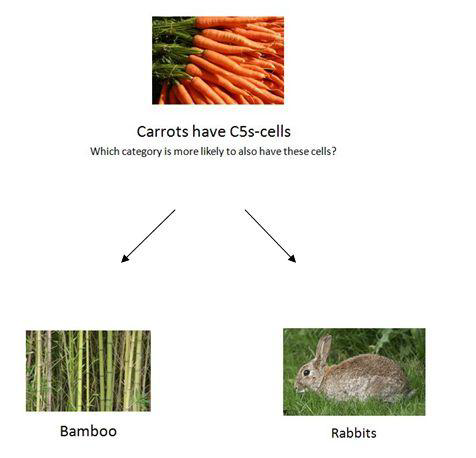
\includegraphics[width=\figurewidth]{imgs/crisp_screenshot.png}
  \caption[
    Screen shot from the triad task used by \citet{Bright}.]{
    \label{fig:crisp_screenshot1}
    Screen shot from the triad task used by \citet{Bright}.
    Participants learned that carrots had a certain property (they had C5s cells),
    and where asked what was most likely to also have that property,
    bamboo, or rabbits.
  }
\end{figure}

While \citegap{Bright}{'s} participants
primarily responded according to structured knowledge,
they were less likely to do so if under heavy cognitive load,
or if lacking in \emph{semantic inhibitory control} \citep{Burgess1997,Markovits2004}.
This last finding, in particular, supports the idea
that reasoning in such contexts involves conflict:
participants responding associatively
were unable to inhibit the
association-driven representation in favour of structured knowledge.

The question remains, however, as to how associative and structure knowledge
actually interact during reasoning.
Later in this chapter, I discuss dual process accounts of reasoning,
where responses can be generated by
two qualitatively different kinds of process:
Type 1, and Type 2 processes.
It should be stressed that \citegap{Bright2014a}{'s} hybrid account
is not a dual process theory, in the sense discussed below.
Rather, it proposes that different kinds of knowledge
differ in the way in which information is represented,
rather than qualitatively in the kinds of process they engage.
With that caveat in place,
much attention \citep[e.g.][]{Evans2007a} has been given to
the issue of how different processes interact in dual process theories.
It is therefore worth considering
how existing ideas about how Type 1 and Type 2 processes interact
might apply to the interaction of different sources of information in induction.

It may be the case that participants draw
on either associative or structured knowledge, for instance, for a given inference.
If this is the case, we would not expect to see
evidence of conflict between different sources of information on a single trial.
Alternatively,
it may be that some sources of information
are available quickly and easily, and so are accessed by default.
In this case, participants may
retrieve such information initially,
but later inhibit it, or at least attempt to inhibit it,
in favour of more useful knowledge,
if they realise their initial source of information
to be inappropriate.
A third possibility is that multiple types of information
are brought to bear simultaneously in parallel.
However, it is difficult to draw predictions from such an account,
and so I will not discuss it further.

This juncture, of course, is not the only point
where conflict can arise in reasoning,
and in fact the issue of conflict is rarely discussed
in the context of induction.
However, in recent years the issue of conflict
has become the focus of attention elsewhere,
by those interested in dual process accounts of reasoning.






% Borrowing from DPT
% - Selective, default, parallel?
% - Stanovich and West
% -> But this ISN'T DPT






